\documentclass[11pt,a4paper]{article}
\usepackage[T1]{fontenc}
\usepackage[utf8]{inputenc}
\usepackage{mathpazo}
\usepackage{microtype}
\usepackage[a4paper,left=2.6cm,right=2.6cm,top=2.7cm,bottom=2.7cm]{geometry}
\usepackage{amsmath,amssymb,amsthm}
\usepackage{xcolor}
\usepackage{booktabs,array}
\usepackage{enumitem}
\usepackage{graphicx}
\usepackage{qrcode}
\usepackage{float}
\usepackage{caption}
\usepackage{fancyhdr}
\usepackage{titlesec}
\usepackage{listings}
\usepackage{algorithm}
\usepackage[noend]{algpseudocode}
\usepackage{tikz}
\usetikzlibrary{arrows.meta,calc,positioning,shapes.geometric,decorations.pathreplacing}
\usepackage{pgfplots}
\pgfplotsset{compat=1.16}

\definecolor{navy}{RGB}{35,55,107}
\definecolor{teal}{RGB}{27,127,117}
\definecolor{slate}{RGB}{107,114,128}
\definecolor{paper}{RGB}{243,245,249}
\definecolor{amber}{RGB}{252,215,110}
\definecolor{alert}{RGB}{178,0,0}

\usepackage[colorlinks=true,linkcolor=navy,citecolor=navy,urlcolor=navy,
  pdftitle={Merge Sort - Design and Analysis of Algorithms},
  pdfauthor={DHAIRYA SINGAL}]{hyperref}

\setlength{\parindent}{1.2em}
\setlength{\parskip}{0.15em}
\linespread{1.04}
\setlist{itemsep=2pt,topsep=3pt}
\captionsetup{font=small,labelfont=bf,labelsep=period}

\titleformat{\section}{\large\bfseries}{\thesection}{0.8em}{}
\titleformat{\subsection}{\normalsize\bfseries}{\thesubsection}{0.7em}{}
\titlespacing*{\section}{0pt}{1.4em}{0.5em}
\titlespacing*{\subsection}{0pt}{1.0em}{0.35em}

\pagestyle{fancy}
\fancyhf{}
\fancyhead[L]{\small\color{slate}Merge Sort}
\fancyhead[R]{\small\color{slate}DHAIRYA SINGAL (590022191)}
\fancyfoot[C]{\small\thepage}
\renewcommand{\headrulewidth}{0.4pt}
\renewcommand{\headrule}{\hbox to\headwidth{\color{navy!60}\leaders\hrule height \headrulewidth\hfill}}

\theoremstyle{plain}
\newtheorem{lemma}{Lemma}
\newtheorem{theorem}{Theorem}
\theoremstyle{definition}
\newtheorem{example}{Example}

\newcommand{\Oh}{\mathcal{O}}
\renewcommand{\lg}{\log_2}

\lstdefinestyle{cstyle}{
  language=C, basicstyle=\ttfamily\footnotesize, keywordstyle=\color{navy}\bfseries,
  commentstyle=\color{slate}\itshape, numbers=left, numberstyle=\tiny\color{slate},
  numbersep=6pt, backgroundcolor=\color{paper}, frame=single, rulecolor=\color{navy!30},
  showstringspaces=false, columns=fullflexible, xleftmargin=1.2em, framexleftmargin=1.2em,
  aboveskip=0.6em, belowskip=0.4em, upquote=true}
\lstset{style=cstyle}

% ---------------- TikZ helpers ----------------
\tikzset{
  abox/.style={draw=navy!70, minimum width=0.72cm, minimum height=0.6cm, inner sep=0pt, font=\small},
  taken/.style={abox, fill=slate!25, text=slate},
  cmp/.style={abox, fill=amber, line width=0.8pt},
  norm/.style={abox, fill=white},
  outb/.style={abox, fill=teal!22, draw=teal},
  emp/.style={abox, dashed, draw=slate!70},
  sbox/.style={draw=navy!70, minimum width=0.62cm, minimum height=0.55cm, inner sep=0pt, font=\small},
  tnode/.style={draw=navy!60, rounded corners=2pt, fill=paper, inner sep=2.5pt, align=center, font=\scriptsize}
}

% one frame of the merge animation: i, j (0-based pointers), k = elements already output
\newcommand{\mframe}[3]{%
\begin{tikzpicture}[x=1cm,y=1cm]
  \def\mi{#1}\def\mj{#2}\def\mk{#3}
  \node[anchor=east,font=\scriptsize\bfseries,color=navy] at (-0.55,2.6) {L};
  \node[anchor=east,font=\scriptsize\bfseries,color=navy] at (-0.55,1.3) {R};
  \node[anchor=east,font=\scriptsize\bfseries,color=teal] at (-0.55,-0.3) {out};
  \foreach \v [count=\c from 0] in {3,27,38,43}{%
    \ifnum\c<\mi \def\st{taken}\else\ifnum\c=\mi\ifnum\mj<3\def\st{cmp}\else\def\st{norm}\fi\else\def\st{norm}\fi\fi
    \node[\st] at (\c*0.8,2.6) {\v};}
  \foreach \v [count=\c from 0] in {9,10,82}{%
    \ifnum\c<\mj \def\st{taken}\else\ifnum\c=\mj\ifnum\mi<4\def\st{cmp}\else\def\st{norm}\fi\else\def\st{norm}\fi\fi
    \node[\st] at (\c*0.8,1.3) {\v};}
  \foreach \v [count=\c from 0] in {3,9,10,27,38,43,82}{%
    \ifnum\c<\mk \def\st{outb}\else\def\st{emp}\fi
    \ifnum\c<\mk\node[\st] at (\c*0.8,-0.3) {\v};\else\node[\st] at (\c*0.8,-0.3) {};\fi}
  \ifnum\mi<4 \node[font=\scriptsize,color=navy] at (\mi*0.8,1.95) {$\uparrow i$};\fi
  \ifnum\mj<3 \node[font=\scriptsize,color=navy] at (\mj*0.8,0.65) {$\uparrow j$};\fi
\end{tikzpicture}}

% one row of the run-snapshot figure: y, label, groups
\newdimen\sx
\newcommand{\snaprow}[4]{%
  \global\sx=0pt
  \node[anchor=east,font=\scriptsize,color=slate] at (-0.25,#1) {#2};
  \foreach \g [count=\gi] in {#3}{%
    \foreach \v in \g {%
      \ifodd\gi \node[sbox,fill=navy!10] at (\the\sx,#1) {\v};%
      \else \node[sbox,fill=teal!18] at (\the\sx,#1) {\v};\fi
      \global\advance\sx by 0.66cm}%
    \global\advance\sx by 0.32cm}%
  \node[anchor=west,font=\scriptsize,color=navy] at (6.45,#1) {#4};}

\begin{document}
\setcounter{page}{0}
% ---------------- COVER ----------------
\begin{titlepage}
\thispagestyle{empty}
\centering
\vspace*{2.2cm}
{\large UPES, \textsc{Dehradun}}\\[0.25em]
{\small School of Computer Science $\cdot$ Artificial Intelligence Cluster}\\[3.6cm]
{\color{navy}\rule{\textwidth}{0.6pt}}\\[1.0cm]
{\color{navy}\bfseries\LARGE Merge Sort}\\[0.6cm]
{\large Mid-Semester Assignment Report}\\[0.9cm]
{\color{navy}\rule{\textwidth}{0.6pt}}\\[1.5cm]
\begin{tabular}{r@{\hspace{0.7em}}l}
\textbf{Course:} & Design and Analysis of Algorithms\\
\textbf{Student:} & DHAIRYA SINGAL\\
\textbf{SAP ID:} & 590022191\\
\textbf{Batch:} & B18\\
\textbf{Semester:} & III (Aug--Dec 2026)\\
\textbf{Submitted to:} & Kunwar Siddharth, Assistant Professor\\
\textbf{Date:} & October 15, 2026
\end{tabular}
\vfill
{\color{navy}\qrcode[height=2.4cm]{https://github.com/DhairyaSingal/merge-animation}}\\[0.2em]
{\scriptsize Scan to open the animation / code}
\vspace*{1.4cm}
\end{titlepage}

% ---------------- ABSTRACT + CONTENTS ----------------
\begin{center}{\large\bfseries Abstract}\end{center}
\begin{quote}\small
Merge sort is a comparison-based sorting algorithm built on divide and conquer: it splits an array into halves, sorts each half recursively, and merges the two sorted halves in linear time. This report explains the intuition behind the method, proves the merge step correct with a loop invariant, and traces the algorithm by hand on a seven-element array. Its running time is then calculated in full: the recurrence $T(n)=2T(n/2)+\Theta(n)$ is solved by the recursion-tree method, verified by substitution and the Master Theorem, and refined to the exact worst-case comparison count $W(n)=n\lceil\lg n\rceil-2^{\lceil\lg n\rceil}+1$; an information-theoretic argument shows that $\Theta(n\log n)$ cannot be beaten by any comparison sort. To make the ideas concrete I built two artefacts: a C implementation with a trace mode and a comparison counter, and an interactive browser animation in which every comparison of the merge step is a separate step and the input array can be edited; four key frames are reproduced in this report. Benchmarks on arrays of up to 100,000 integers show merge sort running about 3,300 times faster than bubble sort, with measured comparison counts that agree with theory. The one idea a reader should keep: merging two sorted lists is cheap, so sorting reduces to repeated cheap merging.
\end{quote}
\vspace{0.3em}
\begingroup
\renewcommand{\contentsname}{\large Contents}
\small
\setcounter{tocdepth}{1}
\tableofcontents
\endgroup
\newpage

% ---------------- 1 ----------------
\section{Introduction}
Sorting arranges a collection of items into a defined order, and it sits underneath many other tasks: searching with binary search, removing duplicates, ranking results, and grouping records. A sorting algorithm is judged by its running time, its extra memory, and whether it is \emph{stable} (items with equal keys keep their original order).

Merge sort was proposed by John von Neumann in 1945 and is one of the first algorithms whose cost was analysed with a recurrence~\cite{knuth3}. It is the standard example of the divide-and-conquer paradigm described in \emph{Introduction to Algorithms} (Cormen, Leiserson, Rivest and Stein)~\cite{clrs}; other textbook treatments are~\cite{sedgewick,kleinberg,dpv}. Unlike quicksort, its running time does not depend on the input order, which makes it predictable and easy to reason about.

This report covers the idea (Section~\ref{sec:intuition}), the mathematics (Section~\ref{sec:math}), the procedure and a hand trace (Sections~\ref{sec:algo}--\ref{sec:example}), the software and animation I built (Section~\ref{sec:demo}), a full calculation of the time and space complexity (Section~\ref{sec:complexity}), an empirical comparison (Section~\ref{sec:empirical}), and where the algorithm is used (Section~\ref{sec:apps}). Sources are listed in the References.

% ---------------- 2 ----------------
\section{Intuition and Core Idea}\label{sec:intuition}
Sorting a long list directly is hard, but two facts make it easy to break down:
\begin{itemize}
  \item A list with \textbf{zero or one} element is already sorted.
  \item Two \textbf{already sorted} lists can be combined into one sorted list very cheaply, because only the front elements ever need to be compared.
\end{itemize}
Think of two sorted piles of exam papers. To produce one sorted pile you repeatedly look at the top paper of each pile, take the one with the smaller roll number, and place it on the output. You never need to look deeper into a pile, so combining $p+q$ papers takes about $p+q$ steps.

Merge sort turns this into three steps:
\begin{enumerate}
  \item \textbf{Divide} the array into two halves.
  \item \textbf{Conquer} by sorting each half recursively (stop at size one).
  \item \textbf{Combine} the sorted halves with the two-pointer merge.
\end{enumerate}
All the real work happens in the combine step; the divide step only computes a midpoint. The recursion therefore has two phases: a \emph{downward} phase that only splits (no comparisons at all) until every piece has one element, and an \emph{upward} phase in which pieces are merged back into longer and longer sorted runs. Figure~\ref{fig:snapshots} later shows both phases on a real array.

% ---------------- 3 ----------------
\section{Mathematical Formulation}\label{sec:math}
\textbf{Problem.} Given $A[1..n]$ drawn from a totally ordered set, produce a permutation $A'$ of $A$ with $A'[1]\le A'[2]\le\dots\le A'[n]$.

\textbf{Merge.} Given sorted sequences $L$ (length $p$) and $R$ (length $q$), produce the sorted sequence of all $p+q$ elements. Every comparison places one element in the output, and the last element is placed without a comparison, so
\begin{equation}
  \mathrm{comparisons}(L,R)\;\le\;p+q-1.
  \label{eq:merge}
\end{equation}

\begin{lemma}[Merge invariant]\label{lem:inv}
At the start of each iteration of the main merge loop, the output holds the $k$ smallest elements of $L\cup R$ in sorted order, and the pointers $i,j$ point at the smallest unused element of $L$ and of $R$ respectively.
\end{lemma}
\begin{proof}
Initially $k=0$ and the claim is trivial. Suppose it holds at some iteration. The smallest unused element of $L\cup R$ is $\min(L[i],R[j])$, since both lists are sorted. The loop appends exactly that element and advances the matching pointer, so the claim holds at the next iteration. When one list is exhausted, the remainder of the other is sorted and larger than everything output, so copying it finishes the merge.
\end{proof}

\noindent\textbf{Correctness of the sort} follows by induction on $n$: the base case $n\le 1$ is trivially sorted; for $n>1$ the two recursive calls sort the halves (induction hypothesis), and the lemma shows the merge of two sorted halves is sorted.

\begin{lemma}[Stability]\label{lem:stab}
If the merge takes the element of $L$ whenever $L[i]\le R[j]$, merge sort is stable.
\end{lemma}
\begin{proof}
Elements of $L$ come from the left half of the array, so equal keys in $L$ originally precede those in $R$. Because ties are resolved in favour of $L$, equal keys leave the merge in the same relative order. Equal keys inside one half keep their order by induction on the recursion depth.
\end{proof}

The running time and space of the algorithm are derived in Section~\ref{sec:complexity}.

% ---------------- 4 ----------------
\section{Algorithm / Procedure}\label{sec:algo}
\begin{algorithm}[!ht]
\caption{\textsc{MergeSort}$(A,lo,hi)$}
\begin{algorithmic}[1]
\Require array $A$, indices $lo\le hi$
\Ensure $A[lo..hi]$ sorted in non-decreasing order
\If{$lo\ge hi$} \Return \Comment{base case: 0 or 1 element}
\EndIf
\State $mid\gets lo+\lfloor (hi-lo)/2\rfloor$
\State \textsc{MergeSort}$(A,lo,mid)$
\State \textsc{MergeSort}$(A,mid+1,hi)$
\State \textsc{Merge}$(A,lo,mid,hi)$
\end{algorithmic}
\end{algorithm}

\begin{algorithm}[!ht]
\caption{\textsc{Merge}$(A,lo,mid,hi)$}
\begin{algorithmic}[1]
\State $i\gets lo,\; j\gets mid+1,\; k\gets lo$; \; $tmp$ is a buffer of the same size as $A$
\While{$i\le mid$ \textbf{and} $j\le hi$}
  \If{$A[i]\le A[j]$}
    \State $tmp[k]\gets A[i];\; i\gets i+1$
  \Else
    \State $tmp[k]\gets A[j];\; j\gets j+1$
  \EndIf
  \State $k\gets k+1$
\EndWhile
\State copy any remaining elements of $A[i..mid]$ or $A[j..hi]$ into $tmp$
\State copy $tmp[lo..hi]$ back into $A[lo..hi]$
\end{algorithmic}
\end{algorithm}

Using $\le$ rather than $<$ on line 3 of \textsc{Merge} makes ties take the left element first, which is exactly what makes merge sort stable (Lemma~\ref{lem:stab}). Computing the midpoint as $lo+\lfloor(hi-lo)/2\rfloor$ avoids integer overflow for very large arrays.

\subsection{Common variants}
\begin{itemize}
  \item \textbf{Bottom-up (iterative) merge sort} starts with runs of length 1 and merges neighbouring runs of length $1,2,4,\dots$ in passes, removing the recursion stack entirely~\cite{sedgewick}.
  \item \textbf{Insertion-sort cutoff.} Below a threshold of roughly 7--20 elements, insertion sort has lower overhead, so recursion stops early and the small block is sorted directly.
  \item \textbf{Natural merge sort} detects runs that are already sorted and merges them, so nearly sorted input is handled in close to linear time; Timsort extends this idea~\cite{peters}.
  \item \textbf{Early exit.} If $A[mid]\le A[mid+1]$ the two halves are already in order and the merge can be skipped.
\end{itemize}

% ---------------- 5 ----------------
\section{Worked Example (Step by Step)}\label{sec:example}
Sort $A=[38,27,43,3,9,82,10]$. Figure~\ref{fig:tree} shows the recursion tree: each node shows its sub-array before sorting (black) and after merging (teal).

\begin{figure}[H]
\centering
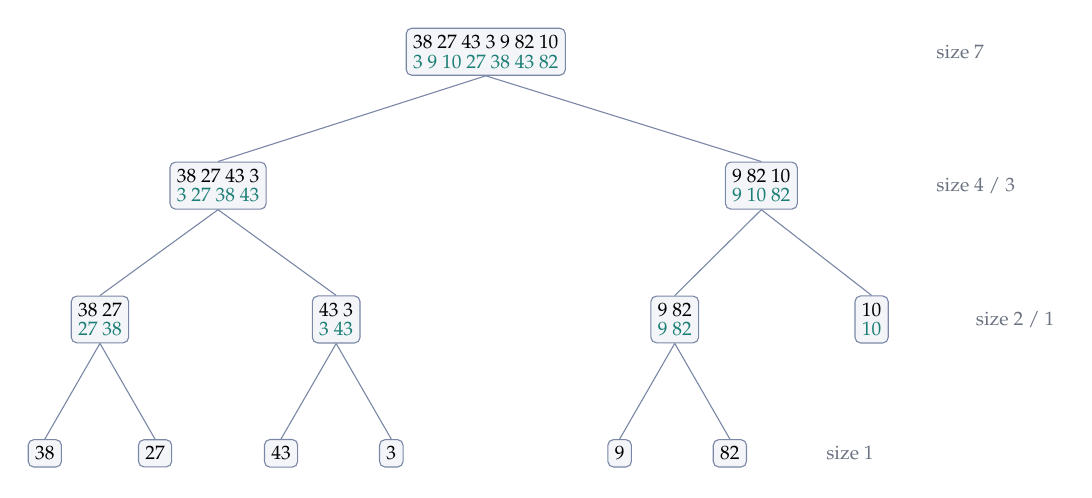
\begin{tikzpicture}[x=1cm,y=1cm]
  \newcommand{\tn}[4]{\ifx\relax#4\relax\node[tnode] (#1) at (#2) {#3};\else\node[tnode] (#1) at (#2) {#3\\[-1pt]\textcolor{teal}{#4}};\fi}
  \tn{r}{5.5,0}{38 27 43 3 9 82 10}{3 9 10 27 38 43 82}
  \tn{a}{2.1,-1.7}{38 27 43 3}{3 27 38 43}
  \tn{b}{9.0,-1.7}{9 82 10}{9 10 82}
  \tn{a1}{0.6,-3.4}{38 27}{27 38}
  \tn{a2}{3.6,-3.4}{43 3}{3 43}
  \tn{b1}{7.9,-3.4}{9 82}{9 82}
  \tn{b2}{10.4,-3.4}{10}{10}
  \tn{l1}{-0.1,-5.1}{38}{}
  \tn{l2}{1.3,-5.1}{27}{}
  \tn{l3}{2.9,-5.1}{43}{}
  \tn{l4}{4.3,-5.1}{3}{}
  \tn{l5}{7.2,-5.1}{9}{}
  \tn{l6}{8.6,-5.1}{82}{}
  \foreach \p/\c in {r/a,r/b,a/a1,a/a2,b/b1,a1/l1,a1/l2,a2/l3,a2/l4,b1/l5,b1/l6}
    \draw[navy!60] (\p.south)--(\c.north);
  \draw[navy!60] (b.south)--(b2.north);
  \node[anchor=west,font=\scriptsize,color=slate] at (11.1,0) {size 7};
  \node[anchor=west,font=\scriptsize,color=slate] at (11.1,-1.7) {size 4 / 3};
  \node[anchor=west,font=\scriptsize,color=slate] at (11.6,-3.4) {size 2 / 1};
  \node[anchor=west,font=\scriptsize,color=slate] at (9.7,-5.1) {size 1};
\end{tikzpicture}
\caption{Recursion tree for $[38,27,43,3,9,82,10]$. Splitting goes downwards; merging returns upwards.}
\label{fig:tree}
\end{figure}

The expensive part is the final merge of $L=[3,27,38,43]$ and $R=[9,10,82]$, traced in Table~\ref{tab:trace}. Seven elements are placed using six comparisons.

\begin{table}[!ht]
\centering\small
\begin{tabular}{@{}clll@{}}
\toprule
Step & Compare $L[i]$ vs $R[j]$ & Take & Output so far\\
\midrule
1 & $3\le 9$   & 3 (L)  & [3]\\
2 & $27>9$     & 9 (R)  & [3, 9]\\
3 & $27>10$    & 10 (R) & [3, 9, 10]\\
4 & $27\le 82$ & 27 (L) & [3, 9, 10, 27]\\
5 & $38\le 82$ & 38 (L) & [3, 9, 10, 27, 38]\\
6 & $43\le 82$ & 43 (L) & [3, 9, 10, 27, 38, 43]\\
7 & $L$ empty  & 82 (R, copy) & [3, 9, 10, 27, 38, 43, 82]\\
\bottomrule
\end{tabular}
\caption{Final merge of $[3,27,38,43]$ and $[9,10,82]$.}
\label{tab:trace}
\end{table}

% ---------------- 6 ----------------
\section{Animation / Software Demonstration}\label{sec:demo}
I built two artefacts: an interactive animation (Section~\ref{sec:anim}) and a C implementation (Section~\ref{sec:csoft}). Section~\ref{sec:diagrams} adds two diagrams drawn in TikZ that mirror the animation.

\subsection{Interactive animation}\label{sec:anim}
Figure~\ref{fig:screens} shows four key frames of the animation running on the example array of Section~\ref{sec:example}.

\begin{figure}[H]
\centering
\begin{minipage}[t]{0.495\textwidth}\centering
\includegraphics[width=\linewidth]{anim_frame1.png}\\[-2pt]{\scriptsize\textbf{Frame 1} (step 1 of 39). Divide: the array is split into two halves; no comparisons yet.}
\end{minipage}\hfill
\begin{minipage}[t]{0.495\textwidth}\centering
\includegraphics[width=\linewidth]{anim_frame2.png}\\[-2pt]{\scriptsize\textbf{Frame 2} (step 33). Final merge: 27 and 10 are compared (yellow) and 10 is taken.}
\end{minipage}\\[1.2em]
\begin{minipage}[t]{0.495\textwidth}\centering
\includegraphics[width=\linewidth]{anim_frame3.png}\\[-2pt]{\scriptsize\textbf{Frame 3} (step 37). The left half is empty, so the leftover 82 is copied without comparing.}
\end{minipage}\hfill
\begin{minipage}[t]{0.495\textwidth}\centering
\includegraphics[width=\linewidth]{anim_frame4.png}\\[-2pt]{\scriptsize\textbf{Frame 4} (step 39). Sorted with 14 comparisons, equal to $W(7)$.}
\end{minipage}
\caption{Screenshots of \texttt{merge\_sort\_animation.html} running on $[38,27,43,3,9,82,10]$.}
\label{fig:screens}
\end{figure}

\textbf{Tool used.} Plain HTML, CSS and JavaScript in a single file, \texttt{merge\_sort\_animation.html}. It uses no libraries and needs no internet connection.

\noindent\textbf{Link.} \url{https://github.com/DhairyaSingal/merge-animation} (code and a copy of this report).

\noindent\textbf{How to run.} Download \texttt{merge\_sort\_animation.html} and open it in any modern browser (Chrome, Edge, Firefox or Safari). Press \emph{Play}, or step with \emph{Next} and \emph{Back} (or the left and right arrow keys); the slider jumps to any step.

\noindent\textbf{What it shows.} When an array is loaded, the program runs merge sort once and records every step. Each step is shown with a sentence explaining it (for example ``Compare 27 and 10: $27>10$, so take 10 from the right half''). The array is drawn as bars: the left half is blue, the right half is green, the pair being compared is yellow, and elements already taken are grey. The pointers $i$ and $j$ sit under the array, the output buffer \texttt{tmp} sits below it, and a counter shows the comparisons so far. At the end the animation reports the final count next to the worst case $W(n)$ of Equation~(\ref{eq:W}).

\noindent\textbf{What the viewer can change.} The input array (2 to 16 whole numbers), the presets \emph{Example}, \emph{Sorted}, \emph{Reversed} and \emph{Random}, and the playback speed. For example, a sorted array of 8 values finishes in 12 comparisons, which is the best-case value $\tfrac12 n\lg n$ in Table~\ref{tab:Wvals}.

\subsection{Merge step diagrams}\label{sec:diagrams}
Figure~\ref{fig:frames} is a TikZ storyboard of the final merge of the worked example. In every frame the highlighted pair is the one being compared, grey boxes have already been taken, and the teal row is the output buffer. Figure~\ref{fig:snapshots} shows the state of the whole array after each level of the recursion, i.e.\ the sequence of runs the animation passes through, together with the number of comparisons spent at each merge level.

\begin{figure}[H]
\centering
\begin{minipage}[t]{0.48\textwidth}\centering
\mframe{0}{0}{0}\\[-1pt]{\scriptsize\textbf{Frame 1.} Pointers at the fronts; compare $3$ and $9$.}
\end{minipage}\hfill
\begin{minipage}[t]{0.48\textwidth}\centering
\mframe{1}{0}{1}\\[-1pt]{\scriptsize\textbf{Frame 2.} $3\le 9$: take $3$ from $L$; compare $27$ and $9$.}
\end{minipage}\\[1.1em]
\begin{minipage}[t]{0.48\textwidth}\centering
\mframe{1}{1}{2}\\[-1pt]{\scriptsize\textbf{Frame 3.} $27>9$: take $9$ from $R$; compare $27$ and $10$.}
\end{minipage}\hfill
\begin{minipage}[t]{0.48\textwidth}\centering
\mframe{1}{2}{3}\\[-1pt]{\scriptsize\textbf{Frame 4.} $27>10$: take $10$ from $R$; compare $27$ and $82$.}
\end{minipage}\\[1.1em]
\begin{minipage}[t]{0.48\textwidth}\centering
\mframe{2}{2}{4}\\[-1pt]{\scriptsize\textbf{Frame 5.} $27\le 82$: take $27$ from $L$; compare $38$ and $82$.}
\end{minipage}\hfill
\begin{minipage}[t]{0.48\textwidth}\centering
\mframe{3}{2}{5}\\[-1pt]{\scriptsize\textbf{Frame 6.} $38\le 82$: take $38$ from $L$; compare $43$ and $82$.}
\end{minipage}\\[1.1em]
\begin{minipage}[t]{0.48\textwidth}\centering
\mframe{4}{2}{6}\\[-1pt]{\scriptsize\textbf{Frame 7.} $43\le 82$: take $43$; $L$ is now empty (6 comparisons used).}
\end{minipage}\hfill
\begin{minipage}[t]{0.48\textwidth}\centering
\mframe{4}{3}{7}\\[-1pt]{\scriptsize\textbf{Frame 8.} Copy the leftover $82$ without comparing; merge complete.}
\end{minipage}
\caption{Storyboard of the two-pointer merge for $L=[3,27,38,43]$ and $R=[9,10,82]$ (one frame per pointer move).}
\label{fig:frames}
\end{figure}

\begin{figure}[H]
\centering
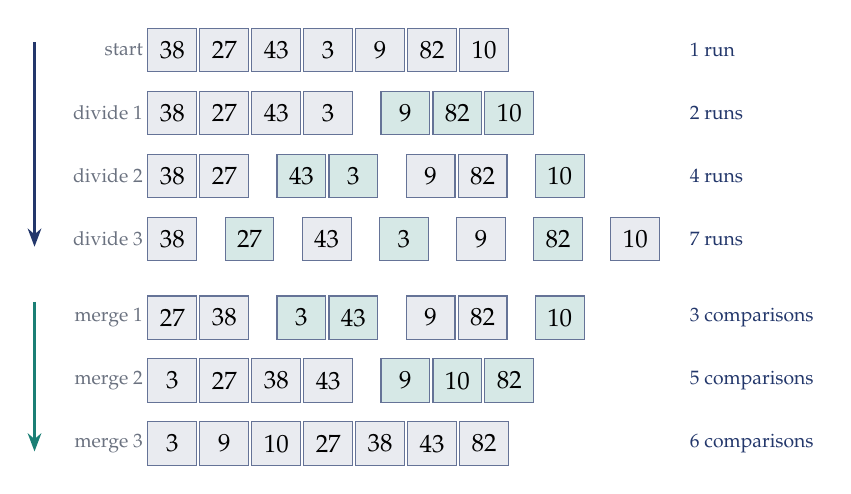
\begin{tikzpicture}[x=1cm,y=1cm]
  \snaprow{0}{start}{{38,27,43,3,9,82,10}}{1 run}
  \snaprow{-0.8}{divide 1}{{38,27,43,3},{9,82,10}}{2 runs}
  \snaprow{-1.6}{divide 2}{{38,27},{43,3},{9,82},{10}}{4 runs}
  \snaprow{-2.4}{divide 3}{{38},{27},{43},{3},{9},{82},{10}}{7 runs}
  \snaprow{-3.4}{merge 1}{{27,38},{3,43},{9,82},{10}}{3 comparisons}
  \snaprow{-4.2}{merge 2}{{3,27,38,43},{9,10,82}}{5 comparisons}
  \snaprow{-5.0}{merge 3}{{3,9,10,27,38,43,82}}{6 comparisons}
  \draw[-{Stealth},navy,thick] (-1.75,0.1)--(-1.75,-2.5);
  \draw[-{Stealth},teal,thick] (-1.75,-3.2)--(-1.75,-5.1);
\end{tikzpicture}
\caption{State of the array after each level. Alternating shades mark separate runs. Divide steps cost no comparisons; the three merge levels cost $3+5+6=14$ comparisons in total.}
\label{fig:snapshots}
\end{figure}

\subsection{The C implementation}\label{sec:csoft}
The recursive driver and the merge step are shown below; the counter \texttt{comparisons} is a global incremented once per element comparison.
\begin{lstlisting}
static long comparisons = 0;

static void merge(int a[], int tmp[], int lo, int mid, int hi)
{
    int i = lo, j = mid + 1, k = lo;
    while (i <= mid && j <= hi) {
        comparisons++;
        if (a[i] <= a[j]) tmp[k++] = a[i++];
        else              tmp[k++] = a[j++];
    }
    while (i <= mid) tmp[k++] = a[i++];   /* leftovers, left  */
    while (j <= hi)  tmp[k++] = a[j++];   /* leftovers, right */
    for (k = lo; k <= hi; k++) a[k] = tmp[k];
}

static void merge_sort(int a[], int tmp[], int lo, int hi)
{
    if (lo >= hi) return;                 /* 0 or 1 element   */
    int mid = lo + (hi - lo) / 2;
    merge_sort(a, tmp, lo, mid);
    merge_sort(a, tmp, mid + 1, hi);
    merge(a, tmp, lo, mid, hi);
}
\end{lstlisting}
Running \texttt{./merge\_sort} on the example array prints the trace below (indentation shows recursion depth) and reports 14 comparisons, the value predicted by $W(7)$ in Section~\ref{sec:complexity}.
\begin{lstlisting}[numbers=none,basicstyle=\ttfamily\scriptsize]
divide [38, 27, 43, 3, 9, 82, 10]
  divide [38, 27, 43, 3]
    divide [38, 27]
    merge  [27, 38]
    divide [43, 3]
    merge  [3, 43]
  merge  [3, 27, 38, 43]
  divide [9, 82, 10]
    divide [9, 82]
    merge  [9, 82]
  merge  [9, 10, 82]
merge  [3, 9, 10, 27, 38, 43, 82]
\end{lstlisting}

% ---------------- 7 ----------------
\section{Time Complexity Analysis}\label{sec:complexity}
This section calculates the cost of merge sort from first principles. Costs are measured in elementary operations (comparisons and element moves), and $\lg=\log_2$.

\subsection{Cost of each step}
\begin{itemize}
  \item \textbf{Divide:} computing $mid$ is a constant number of operations, $\Theta(1)$.
  \item \textbf{Conquer:} two recursive calls on subarrays of sizes $\lceil n/2\rceil$ and $\lfloor n/2\rfloor$.
  \item \textbf{Combine:} \textsc{Merge} on $m$ elements makes at most $m-1$ comparisons (Equation~\ref{eq:merge}), writes every element once into $tmp$ ($m$ moves) and copies it back ($m$ moves). Because the two copy loops always run, \textsc{Merge} costs $\Theta(m)$ \emph{whatever the data are}; write its cost as at most $c\,m$ for a constant $c$.
\end{itemize}
Let $T(n)$ be the running time on $n$ elements and let $c_0$ be the constant cost of the base case. Then
\begin{equation}
  T(n)=T(\lceil n/2\rceil)+T(\lfloor n/2\rfloor)+cn,\qquad T(1)=c_0.
  \label{eq:rec}
\end{equation}
For the calculations below take $n=2^k$, so that both halves have exactly $n/2$ elements and $T(n)=2T(n/2)+cn$.

\subsection{Solving by the recursion-tree method}
Expand the recursion level by level (Figure~\ref{fig:cost}). At depth $i$ there are $2^i$ subproblems, each of size $n/2^i$, and each one pays a merge cost of $c\,n/2^i$. The cost of level $i$ is therefore
\[
  2^i\cdot c\,\frac{n}{2^i}=cn,
\]
the same at every level. Table~\ref{tab:levels} lists the levels.

\begin{table}[!ht]
\centering\small
\begin{tabular}{@{}cccccc@{}}
\toprule
Depth $i$ & Subproblems & Size each & Merge cost each & Cost of level\\
\midrule
0 & $1$ & $n$ & $cn$ & $cn$\\
1 & $2$ & $n/2$ & $cn/2$ & $cn$\\
2 & $4$ & $n/4$ & $cn/4$ & $cn$\\
$\vdots$ & $\vdots$ & $\vdots$ & $\vdots$ & $\vdots$\\
$i$ & $2^i$ & $n/2^i$ & $cn/2^i$ & $cn$\\
$\vdots$ & $\vdots$ & $\vdots$ & $\vdots$ & $\vdots$\\
$k-1$ & $n/2$ & $2$ & $2c$ & $cn$\\
$k=\lg n$ (leaves) & $n$ & $1$ & $c_0$ & $c_0n$\\
\bottomrule
\end{tabular}
\caption{Cost of each level of the recursion tree for $n=2^k$.}
\label{tab:levels}
\end{table}

\begin{figure}[H]
\centering
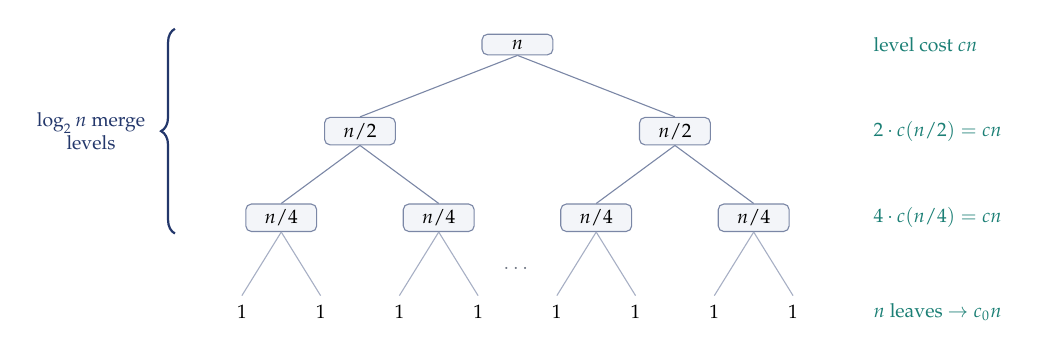
\begin{tikzpicture}[x=1cm,y=1cm]
  \tikzset{n/.style={draw=navy!60,rounded corners=2pt,fill=paper,inner sep=2pt,font=\scriptsize,minimum width=0.9cm}}
  \node[n] (r) at (4,0) {$n$};
  \node[n] (a) at (2,-1.1) {$n/2$};
  \node[n] (b) at (6,-1.1) {$n/2$};
  \foreach \x/\p in {1/a,3/a,5/b,7/b}{\node[n] (c\x) at (\x,-2.2) {$n/4$}; \draw[navy!60] (\p.south)--(c\x.north);}
  \draw[navy!60] (r.south)--(a.north); \draw[navy!60] (r.south)--(b.north);
  \foreach \li in {1,...,8}{\node[font=\scriptsize] (l\li) at (\li-0.5,-3.4) {$1$};}
  \foreach \li/\p in {1/1,2/1,3/3,4/3,5/5,6/5,7/7,8/7}{\draw[navy!40] (c\p.south)--(l\li.north);}
  \node[font=\scriptsize,color=slate] at (4,-2.85) {$\cdots$};
  \node[anchor=west,font=\scriptsize,color=teal] at (8.4,0) {level cost $cn$};
  \node[anchor=west,font=\scriptsize,color=teal] at (8.4,-1.1) {$2\cdot c(n/2)=cn$};
  \node[anchor=west,font=\scriptsize,color=teal] at (8.4,-2.2) {$4\cdot c(n/4)=cn$};
  \node[anchor=west,font=\scriptsize,color=teal] at (8.4,-3.4) {$n$ leaves $\to c_0n$};
  \draw[decorate,decoration={brace,amplitude=5pt,mirror},navy,thick] (-0.35,0.2)--(-0.35,-2.4) node[midway,left=7pt,font=\scriptsize,align=center]{$\lg n$ merge\\levels};
\end{tikzpicture}
\caption{Recursion tree of merge sort. Every merge level costs $cn$, and there are $\lg n$ of them.}
\label{fig:cost}
\end{figure}

Adding the $k=\lg n$ merge levels and the leaves gives
\[
  T(n)=\sum_{i=0}^{k-1}cn+c_0n=cn\lg n+c_0n=\Theta(n\log n),
\]
because for large $n$ the term $cn\lg n$ dominates $c_0n$.

\subsection{Verification by substitution}
\begin{theorem}\label{thm:subst}
For $n=2^k$, the recurrence $T(n)=2T(n/2)+cn$, $T(1)=c_0$ has the solution $T(n)=cn\lg n+c_0n$.
\end{theorem}
\begin{proof}
Induction on $k$. For $k=0$: $T(1)=c_0=c\cdot1\cdot0+c_0\cdot1$. Assume $T(2^{k-1})=c2^{k-1}(k-1)+c_02^{k-1}$. Then
\begin{align*}
T(2^k)&=2\,T(2^{k-1})+c2^k\\
&=2\bigl[c2^{k-1}(k-1)+c_02^{k-1}\bigr]+c2^k\\
&=c2^k(k-1)+c_02^k+c2^k=c2^kk+c_02^k. \qedhere
\end{align*}
\end{proof}

\subsection{Verification by the Master Theorem}
The Master Theorem~\cite{clrs,bentley} solves $T(n)=aT(n/b)+f(n)$ by comparing $f(n)$ with $n^{\log_ba}$. Here $a=2$, $b=2$, so $n^{\log_ba}=n^{\log_22}=n$ and $f(n)=cn=\Theta(n)=\Theta\bigl(n^{\log_ba}\bigr)$. This is Case~2, hence
\[
  T(n)=\Theta\bigl(n^{\log_ba}\log n\bigr)=\Theta(n\log n).
\]
All three methods agree.

\subsection{Arbitrary $n$}
If $n$ is not a power of two choose $k$ with $2^{k-1}<n\le2^k$. The merge cost grows with the size of the subarray, so $T$ is non-decreasing and
\[
  T(2^{k-1})\le T(n)\le T(2^k).
\]
Both ends are $\Theta(2^k k)$ and $2^{k-1}<n\le2^k$ gives $2^k<2n$ and $k<\lg n+1$, so $T(n)=\Theta(n\log n)$ for every $n$.

\subsection{Exact number of comparisons}
Counting only comparisons, the worst case satisfies
\[
  W(n)=W(\lceil n/2\rceil)+W(\lfloor n/2\rfloor)+(n-1),\qquad W(1)=0,
\]
since a merge of $n$ elements needs at most $n-1$ comparisons. The closed form is
\begin{equation}
  W(n)=n\lceil\lg n\rceil-2^{\lceil\lg n\rceil}+1.
  \label{eq:W}
\end{equation}
\emph{Proof for $n=2^k$.} Here $W(2^k)=2W(2^{k-1})+2^k-1$. Assuming $W(2^{k-1})=(k-1)2^{k-1}-2^{k-1}+1$,
\[
  W(2^k)=(k-1)2^k-2^k+2+2^k-1=k2^k-2^k+1,
\]
which is (\ref{eq:W}) with $\lceil\lg n\rceil=k$. The case of general $n$ is proved in~\cite{knuth3}.

\medskip\noindent\textbf{Check on the worked example.} For $n=7$, Equation~(\ref{eq:W}) gives $W(7)=7\cdot3-8+1=14$. Table~\ref{tab:n7} confirms this by adding the worst case of every merge in the recursion tree of Figure~\ref{fig:tree}. The C program reports exactly 14 comparisons on this array, which therefore happens to be a worst case.

\begin{table}[!ht]
\centering\small
\begin{tabular}{@{}cllc@{}}
\toprule
Depth & Merges (sizes) & Comparisons per merge & Total\\
\midrule
2 & three merges of size 2 & $1,1,1$ & 3\\
1 & sizes 4 ($2+2$) and 3 ($2+1$) & $3,\;2$ & 5\\
0 & one merge of size 7 ($4+3$) & $6$ & 6\\
\midrule
\multicolumn{3}{r}{Total $=W(7)$} & \textbf{14}\\
\bottomrule
\end{tabular}
\caption{Worst-case comparisons for the seven-element example, level by level.}
\label{tab:n7}
\end{table}

\subsection{Best, average and worst case}
For $n=2^k$ the quantities of interest are collected in Table~\ref{tab:cases}.
\begin{table}[!ht]
\centering\small
\begin{tabular}{@{}lccc@{}}
\toprule
Case & Comparisons & Element moves & Running time\\
\midrule
Best (already sorted) & $\tfrac12 n\lg n$ & $2n\lg n$ & $\Theta(n\log n)$\\
Average (random) & $\approx n\lg n-1.25\,n$ & $2n\lg n$ & $\Theta(n\log n)$\\
Worst & $n\lg n-n+1$ & $2n\lg n$ & $\Theta(n\log n)$\\
\bottomrule
\end{tabular}
\caption{Cost of merge sort for $n=2^k$.}
\label{tab:cases}
\end{table}
In the best case every merge ends after exhausting the shorter list, costing $n/2$ comparisons per level instead of $n-1$. The number of \emph{moves} does not depend on the data (each level moves $n$ elements into $tmp$ and $n$ back), so the running time is $\Theta(n\log n)$ in all three cases. This is the practical advantage over quicksort, whose worst case is $\Theta(n^2)$. The average comparison count is approximately $n\lg n-1.25n$~\cite{knuth3,flajolet}. Table~\ref{tab:Wvals} gives exact values.

\begin{table}[!ht]
\centering\small
\begin{tabular}{@{}rrrrr@{}}
\toprule
$n$ & Best $\tfrac12 n\lg n$ & Worst $W(n)$ & $n\lg n$ & Lower bound $\lceil\lg n!\rceil$\\
\midrule
2 & 1 & 1 & 2 & 1\\
4 & 4 & 5 & 8 & 5\\
8 & 12 & 17 & 24 & 16\\
16 & 32 & 49 & 64 & 45\\
64 & 192 & 321 & 384 & 296\\
256 & 1,024 & 1,793 & 2,048 & 1,684\\
1,024 & 5,120 & 9,217 & 10,240 & 8,770\\
\bottomrule
\end{tabular}
\caption{Exact comparison counts for powers of two, and the information-theoretic lower bound of Section~\ref{sec:lower}.}
\label{tab:Wvals}
\end{table}

\subsection{Space complexity}
\textsc{Merge} needs a buffer $tmp$ of up to $n$ elements, which is allocated once and reused, so the auxiliary array costs $\Theta(n)$. The recursion depth is $\lceil\lg n\rceil+1$ because the range halves at each call, adding $\Theta(\log n)$ for the call stack. The total auxiliary space is therefore $\Theta(n)+\Theta(\log n)=\Theta(n)$.

\subsection{Why $\Theta(n\log n)$ is optimal}\label{sec:lower}
Any comparison sort can be drawn as a binary decision tree whose leaves are the $n!$ possible orderings of the input. A binary tree with $n!$ leaves has height at least $\lg(n!)$, and since $n!\ge(n/e)^n$,
\[
  \lg(n!)\ge n\lg n-n\lg e\approx n\lg n-1.44\,n.
\]
So every comparison sort needs $\Omega(n\log n)$ comparisons in the worst case~\cite{clrs}. Merge sort matches this bound, so it is asymptotically optimal, and for $n=7$ the bound is $\lceil\lg 5040\rceil=\lceil12.30\rceil=13$ against merge sort's $14$.

\subsection{What the formulas mean in practice}
Table~\ref{tab:model} converts the operation counts into time on a machine that performs $10^8$ simple operations per second (a deliberately crude model: one operation per comparison). The ratio $n^2/(n\lg n)=n/\lg n$ shows how much a quadratic algorithm falls behind as $n$ grows.
\begin{table}[!ht]
\centering\small
\begin{tabular}{@{}rrrrrr@{}}
\toprule
$n$ & $n\lg n$ & $n^2$ & $n\lg n$ time & $n^2$ time & $n/\lg n$\\
\midrule
$10^3$ & $1.0\times10^4$ & $10^6$ & 0.1 ms & 10 ms & 100\\
$10^4$ & $1.3\times10^5$ & $10^8$ & 1.3 ms & 1 s & 753\\
$10^5$ & $1.7\times10^6$ & $10^{10}$ & 16.6 ms & 100 s & 6,021\\
$10^6$ & $2.0\times10^7$ & $10^{12}$ & 0.2 s & 2.8 h & 50,172\\
$10^7$ & $2.3\times10^8$ & $10^{14}$ & 2.3 s & 11.6 days & 430,043\\
\bottomrule
\end{tabular}
\caption{Predicted running times at $10^8$ operations per second.}
\label{tab:model}
\end{table}

% ---------------- 8 ----------------
\section{Empirical Analysis}\label{sec:empirical}
\subsection{Theoretical comparison}
\begin{table}[!ht]
\centering\small
\begin{tabular}{@{}lccccc@{}}
\toprule
Algorithm & Best & Average & Worst & Space & Stable\\
\midrule
Merge sort & $n\log n$ & $n\log n$ & $n\log n$ & $n$ & Yes\\
Quick sort & $n\log n$ & $n\log n$ & $n^2$ & $\log n$ & No\\
Heap sort & $n\log n$ & $n\log n$ & $n\log n$ & $1$ & No\\
Insertion sort & $n$ & $n^2$ & $n^2$ & $1$ & Yes\\
Bubble sort & $n$ & $n^2$ & $n^2$ & $1$ & Yes\\
\bottomrule
\end{tabular}
\caption{Asymptotic behaviour of common comparison sorts.}
\label{tab:cmp}
\end{table}

\subsection{Empirical results}
I ran the benchmark in \texttt{merge\_sort.c} on random integers (fixed seed 42, single run per size, compiled with \texttt{gcc -O2}). Absolute times depend on the machine; the trend does not (Figure~\ref{fig:plot}).
\begin{table}[!ht]
\centering\small
\begin{tabular}{@{}rrrrr@{}}
\toprule
$n$ & Merge (s) & Bubble (s) & Merge comparisons & \% of $n\lg n$\\
\midrule
1,000 & 0.00009 & 0.00211 & 8,710 & 87.4\\
5,000 & 0.00041 & 0.05151 & 55,245 & 89.9\\
10,000 & 0.00091 & 0.21169 & 120,525 & 90.7\\
50,000 & 0.00496 & 7.83793 & 718,396 & 92.0\\
100,000 & 0.01018 & 33.56811 & 1,536,507 & 92.5\\
\bottomrule
\end{tabular}
\caption{Measured runtime and comparison counts.}
\label{tab:meas}
\end{table}

\begin{figure}[H]
\centering
\begin{minipage}{0.49\textwidth}\centering
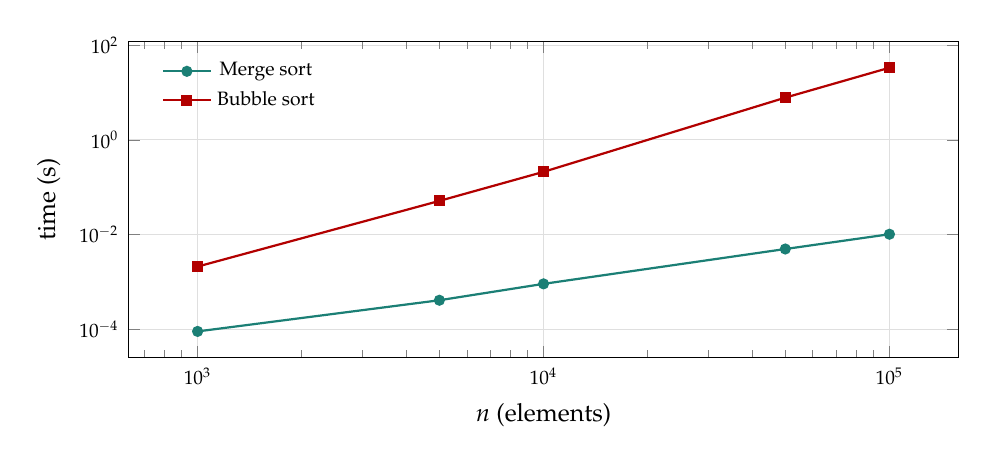
\begin{tikzpicture}
\begin{axis}[width=\linewidth,height=5.6cm,xmode=log,ymode=log,xlabel={$n$ (elements)},ylabel={time (s)},
  grid=major,grid style={gray!25},legend pos=north west,legend style={font=\scriptsize,draw=none,fill=none},
  tick label style={font=\scriptsize},label style={font=\small}]
\addplot[teal,thick,mark=*,mark size=1.6pt] coordinates {(1000,0.00009)(5000,0.00041)(10000,0.00091)(50000,0.00496)(100000,0.01018)};
\addplot[alert,thick,mark=square*,mark size=1.6pt] coordinates {(1000,0.00211)(5000,0.05151)(10000,0.21169)(50000,7.83793)(100000,33.56811)};
\legend{Merge sort,Bubble sort}
\end{axis}
\end{tikzpicture}
\end{minipage}\hfill
\begin{minipage}{0.49\textwidth}\centering
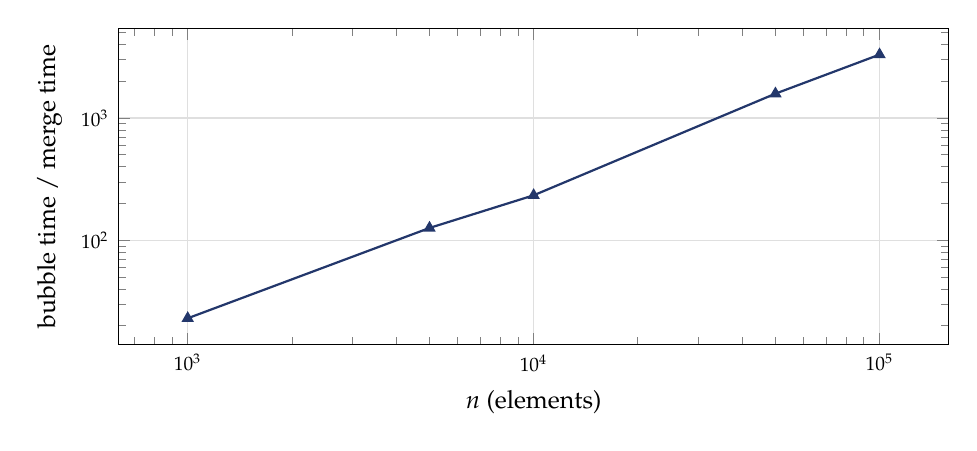
\begin{tikzpicture}
\begin{axis}[width=\linewidth,height=5.6cm,xmode=log,ymode=log,xlabel={$n$ (elements)},ylabel={bubble time / merge time},
  grid=major,grid style={gray!25},tick label style={font=\scriptsize},label style={font=\small}]
\addplot[navy,thick,mark=triangle*,mark size=1.8pt] coordinates {(1000,23)(5000,126)(10000,233)(50000,1580)(100000,3297)};
\end{axis}
\end{tikzpicture}
\end{minipage}
\caption{Left: runtime versus input size on log--log axes. The bubble-sort line is steeper (slope about 2, i.e.\ $n^2$) than the merge-sort line (slope close to 1). Right: the speed-up of merge sort over bubble sort keeps growing with $n$.}
\label{fig:plot}
\end{figure}

\subsection{Measured comparisons against theory}
Table~\ref{tab:thy} sets the measured counts beside the exact worst case from Equation~(\ref{eq:W}) and the average-case estimate $n\lg n-1.25n$.
\begin{table}[!ht]
\centering\small
\begin{tabular}{@{}rrrrr@{}}
\toprule
$n$ & Measured & Worst $W(n)$ & Estimate $n\lg n-1.25n$ & Error vs.\ estimate\\
\midrule
1,000 & 8,710 & 8,977 & 8,716 & $-0.07\%$\\
5,000 & 55,245 & 56,809 & 55,189 & $+0.10\%$\\
10,000 & 120,525 & 123,617 & 120,377 & $+0.12\%$\\
50,000 & 718,396 & 734,465 & 717,982 & $+0.06\%$\\
100,000 & 1,536,507 & 1,568,929 & 1,535,964 & $+0.04\%$\\
\bottomrule
\end{tabular}
\caption{Measured comparison counts, the exact worst case, and the average-case estimate.}
\label{tab:thy}
\end{table}

\subsection{Discussion}
At $n=100{,}000$ merge sort took 0.010~s against 33.6~s for bubble sort, a factor of about 3,300. The gap widens with $n$ because $n^2/(n\lg n)=n/\lg n$ grows without bound.

The measured comparison counts stay below $n\lg n$ and below the worst case $W(n)$ in every row (about 97--98\% of it). This is expected: merging stops comparing as soon as one half runs out, and the average count is close to $n\lg n-1.25n$. For $n=100{,}000$ that estimate is $1{,}660{,}964-125{,}000\approx1{,}535{,}964$, within 0.04\% of the measured $1{,}536{,}507$. The practical cost of merge sort is the $O(n)$ extra buffer, and for very small subarrays the recursion overhead makes insertion sort faster, which is why library implementations combine the two.

% ---------------- 9 ----------------
\section{Applications}\label{sec:apps}
\begin{itemize}
  \item \textbf{Library sorts.} Python's \texttt{sorted} and Java's object sort use Timsort, a hybrid of merge sort and insertion sort that relies on merge sort's stability~\cite{peters}.
  \item \textbf{External sorting.} When data does not fit in memory, sorted chunks are written to disk and then merged; this is how databases sort large tables~\cite{knuth3}.
  \item \textbf{Linked lists.} Merge needs only sequential access and no random indexing, so it is the preferred sort for linked lists.
  \item \textbf{Counting inversions.} A small change to the merge step counts out-of-order pairs in $O(n\log n)$, used in rank-correlation measures~\cite{clrs}.
  \item \textbf{Machine learning pipelines.} Exact split search in decision trees sorts each feature's values~\cite{cart}, ranking and top-$k$ retrieval sort model scores, and distributed frameworks merge sorted partitions from many workers.
  \item \textbf{Parallel computing.} The two recursive calls are independent, so they can run on separate cores or machines.
\end{itemize}

% ---------------- 10 ----------------
\section{Conclusion}
Merge sort reduces a hard problem to repeated easy ones: a one-element array is sorted, and two sorted arrays merge in linear time. This gives $\Theta(n\log n)$ time in every case, stability, and a clean correctness proof, at the price of $O(n)$ extra space. The complexity was calculated three ways (recursion tree, substitution and Master Theorem), refined to the exact count $W(n)=n\lceil\lg n\rceil-2^{\lceil\lg n\rceil}+1$, and shown to be optimal among comparison sorts. My C implementation and the benchmark confirmed the theory: comparison counts track $n\lg n-1.25n$, and merge sort was about 3,300 times faster than bubble sort at $n=100{,}000$. The animation made the two-pointer merge, the only non-obvious step, visible one comparison at a time. Possible extensions are a bottom-up (iterative) version, switching to insertion sort for tiny subarrays, and a parallel implementation.

\section*{Declaration of AI Tool Use}
\addcontentsline{toc}{section}{Declaration of AI Tool Use}
I used an AI assistant (Claude, by Anthropic) to help draft the structure of this report, the C program, and the browser animation. I ran the C program myself, and the figures in Section~\ref{sec:empirical} are the output of that run. I have read the report, checked the mathematics and code, and I understand the algorithm well enough to explain and modify it. Any errors that remain are my own responsibility.

\addcontentsline{toc}{section}{References}
\begin{thebibliography}{99}\small
\setlength{\itemsep}{2pt}
\bibitem{clrs} T.~H. Cormen, C.~E. Leiserson, R.~L. Rivest and C. Stein, \emph{Introduction to Algorithms}, 4th ed., MIT Press, 2022 (Chapter 2: merge sort; Chapter 4: divide-and-conquer and the Master Theorem; Chapter 8: lower bounds for sorting).
\bibitem{knuth3} D.~E. Knuth, \emph{The Art of Computer Programming, Vol.~3: Sorting and Searching}, 2nd ed., Addison-Wesley, 1998 (Section 5.2.4: Sorting by merging; Section 5.4: External sorting).
\bibitem{sedgewick} R. Sedgewick and K. Wayne, \emph{Algorithms}, 4th ed., Addison-Wesley, 2011 (Section 2.2: Mergesort).
\bibitem{kleinberg} J. Kleinberg and \'E. Tardos, \emph{Algorithm Design}, Pearson/Addison-Wesley, 2005 (Chapter 5: Divide and conquer).
\bibitem{dpv} S. Dasgupta, C.~H. Papadimitriou and U. Vazirani, \emph{Algorithms}, McGraw-Hill, 2008 (Chapter 2: Divide-and-conquer algorithms).
\bibitem{bentley} J.~L. Bentley, D. Haken and J.~B. Saxe, ``A general method for solving divide-and-conquer recurrences,'' \emph{ACM SIGACT News}, vol.~12, no.~3, pp.~36--44, 1980.
\bibitem{flajolet} P. Flajolet and M. Golin, ``Mellin transforms and asymptotics: the mergesort recurrence,'' \emph{Acta Informatica}, vol.~31, no.~7, pp.~673--696, 1994.
\bibitem{peters} T. Peters, ``Timsort'' description (\texttt{listsort.txt}), CPython source repository, 2002.
\bibitem{kr} B.~W. Kernighan and D.~M. Ritchie, \emph{The C Programming Language}, 2nd ed., Prentice Hall, 1988.
\bibitem{cart} L. Breiman, J.~H. Friedman, R.~A. Olshen and C.~J. Stone, \emph{Classification and Regression Trees}, Wadsworth, 1984.
\end{thebibliography}

\end{document}
